\documentclass{article}
\usepackage{graphicx} % Required for inserting images
\usepackage{float}
\usepackage[T1]{fontenc}
\usepackage{amsmath}
\usepackage[margin=1in]{geometry}
\usepackage{booktabs}
\usepackage{tabularx}
\usepackage[hidelinks]{hyperref}

\title{Cutting the stress-sized put book on calm-VVIX days}
\author{Experiment report \textperiodcentered{} L/S Gamma Desk, QUANTT}
\date{2026-11-02}

\begin{document}

\maketitle

\textbf{Question:} On the 35\% stress-sized \texttt{hedged} book, does cutting each entry's stress budget on calm-VVIX days (0.5x at VVIX's one-year low, rising to 1x at the median and capped there) give a higher Sharpe ratio than the fixed 35\% budget, over the full window and in each half, with a less severe maximum drawdown, at 1x and 2x spreads?

\textbf{Method:}

\begin{itemize}

\item \textbf{Pre-registration:} the hypothesis card was committed before any run (commit 6eae543). The new research switch \texttt{size\_\allowbreak{}cap} was committed before it, in a2d5334.

\item \textbf{Data:} the live paper rules (\texttt{configs/\allowbreak{}paper.\allowbreak{}toml}) are replayed on R2 replay snapshots v1 (config\_hash b040760187f0) over the development window 2014-06-02 to 2024-12-31. The hold-out (2025-01-01 to 2026-07-10) was not used.

\item \textbf{Book:} every variant is the \texttt{hedged} book of 2026-10-22-stress-sized-puts.

\begin{itemize}

\item An always-on short 25-delta put, with the signal ignored and the flat exit off.

\item Sized at each entry to the most contracts whose loss in a one-day 20\% SPY drop, with IV at max(60\%, the put's IV), stays within the budget.

\item Hedged daily with a 10-share band. Stop at 1x the credit, profit-take at 50\% and time exit at 7 DTE.

\end{itemize}

\item \textbf{Capped tilt:} the budget is 35\% \ensuremath{\times} min(1, 1 + tilt \ensuremath{\times} (2p \ensuremath{-} 1)), where p is the percentile of the prior day's VVIX close among its last 252 closes.

\item \textbf{Variants:}

\begin{itemize}

\item \texttt{vvix\_\allowbreak{}cap} (primary): tilt 0.5, cap 1, a budget of 17.5\% to 35\% of capital;

\item \texttt{vvix\_\allowbreak{}cap\_\allowbreak{}light}: tilt 0.25, cap 1, a budget of 26.25\% to 35\%.

\end{itemize}

\item \textbf{Comparison:} the registered \texttt{2026-\allowbreak{}10-\allowbreak{}22-\allowbreak{}stress-\allowbreak{}sized-\allowbreak{}puts/\allowbreak{}hedged} runs at the same spread multiple, reused and not rerun. With the new switches off, the engine reproduces that book's equity exactly.

\item \textbf{Context (charts only):} the uncapped \texttt{2026-\allowbreak{}11-\allowbreak{}02-\allowbreak{}vvix-\allowbreak{}sizing/\allowbreak{}vvix} runs, labelled \texttt{vvix\_\allowbreak{}ref}.

\item \textbf{Costs and schedule:} every variant was run at 1x and 2x spreads. \$0.65 per contract and \$0.005 per share, with a \$1 minimum per order. Decisions, exits and hedges run once a day at 10:15 ET.

\end{itemize}

This report was written by Claude at the PM's request.

\section{Result vs the pass bar}

Every check had to hold at 1x and 2x. Sharpe is annualised from daily net P\&L. Drawdown is the largest fall in cumulative net P\&L from a previous high, in USD.

\begin{center}\small
\begin{tabularx}{\linewidth}{>{\raggedright\arraybackslash}X l l l l >{\raggedright\arraybackslash}X}
\toprule
\textbf{Check (\texttt{vvix\_\allowbreak{}cap} vs \texttt{hedged})} & \textbf{1x value} & \textbf{1x bar} & \textbf{2x value} & \textbf{2x bar} & \textbf{Result} \\
\midrule
Sharpe, full window & 0.48 & > 0.52 & 0.44 & > 0.43 & \textbf{fail (1x)} \\
Sharpe, 2014-06 to 2019-12 & 0.66 & > 0.84 & 0.73 & > 0.72 & \textbf{fail (1x)} \\
Sharpe, 2020-01 to 2024-12 & 0.49 & > 0.48 & 0.41 & > 0.38 & pass \\
Max drawdown less severe & \$74,926 & < \$70,362 & \$74,317 & < \$75,488 & \textbf{fail (1x)} \\
Round trips (floor \ensuremath{\geq} 30) & 182 &  &  &  & met \\
\bottomrule
\end{tabularx}
\end{center}

\textbf{Verdict: failed.} The cap did what it was built to do in calm markets: it made the book smaller.

\begin{itemize}

\item At 1x it lowered the Sharpe ratio, mostly in 2014-2019, and made the drawdown \$4.6k deeper.

\item It passed every check at 2x, but by small margins that come from a different trade path, not from the rule.

\item The book still makes money (\$109k at 1x, \$100k at 2x), but less than the fixed budget.

\end{itemize}

\subsection{Full-window numbers (not part of the bar)}

\begin{center}\small
\begin{tabularx}{\linewidth}{>{\raggedright\arraybackslash}X >{\raggedright\arraybackslash}X >{\raggedright\arraybackslash}X >{\raggedright\arraybackslash}X >{\raggedright\arraybackslash}X >{\raggedright\arraybackslash}X >{\raggedright\arraybackslash}X}
\toprule
\textbf{} & \textbf{\texttt{hedged} 1x} & \textbf{\texttt{vvix\_\allowbreak{}cap} 1x} & \textbf{\texttt{vvix\_\allowbreak{}cap\_\allowbreak{}light} 1x} & \textbf{\texttt{hedged} 2x} & \textbf{\texttt{vvix\_\allowbreak{}cap} 2x} & \textbf{\texttt{vvix\_\allowbreak{}cap\_\allowbreak{}light} 2x} \\
\midrule
Net P\&L & \$121,482 & \$109,430 & \$113,790 & \$101,172 & \$100,144 & \$104,136 \\
Sharpe & 0.52 & 0.48 & 0.49 & 0.43 & 0.44 & 0.45 \\
Max drawdown & \$70,362 & \$74,926 & \$76,935 & \$75,488 & \$74,317 & \$74,909 \\
ES 5\% (daily) & \ensuremath{-}\$3,016 & \ensuremath{-}\$2,761 & \ensuremath{-}\$2,874 & \ensuremath{-}\$3,094 & \ensuremath{-}\$2,788 & \ensuremath{-}\$2,909 \\
Round trips & 182 & 182 & 184 & 181 & 180 & 181 \\
Commissions (options /\allowbreak{} hedges) & \$5,955 /\allowbreak{} \$2,868 & \$5,330 /\allowbreak{} \$2,736 & \$5,692 /\allowbreak{} \$2,802 & \$5,918 /\allowbreak{} \$2,863 & \$5,236 /\allowbreak{} \$2,729 & \$5,580 /\allowbreak{} \$2,792 \\
\bottomrule
\end{tabularx}
\end{center}

The sensitivity \texttt{vvix\_\allowbreak{}cap\_\allowbreak{}light} behaved like the primary: Sharpe 0.49 against 0.52 at 1x and a deeper 1x drawdown (\$76,935). It also fails the bar.

\section{Charts}

\begin{figure}[H]\centering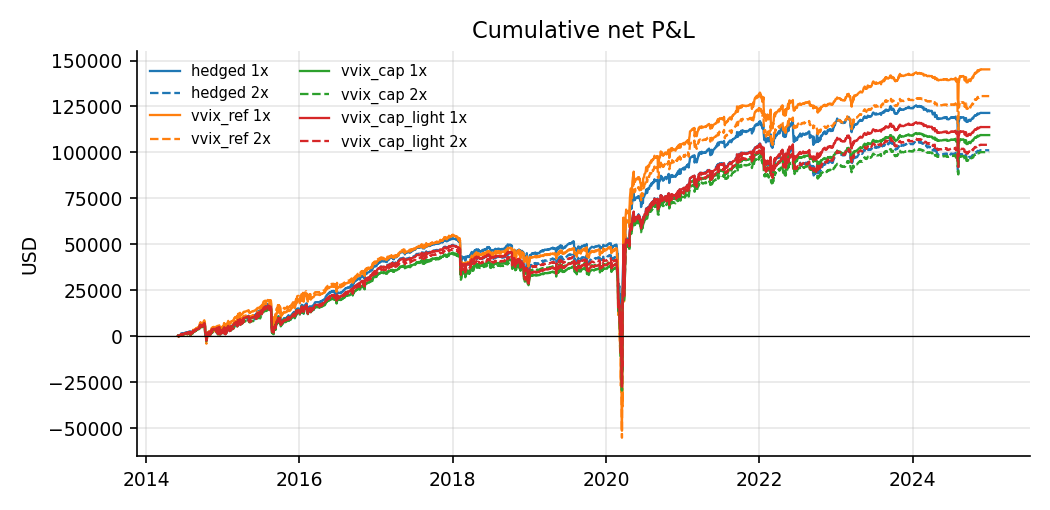
\includegraphics[width=0.92\linewidth]{figures/cum_pnl.png}\caption{Cumulative net P\&L, 1x solid and 2x dashed}\end{figure}

The capped books track the fixed budget closely and sit a little below it from 2016 on. The March 2020 drop is the same size in all three. The uncapped tilt (\texttt{vvix\_\allowbreak{}ref}) is the only line that falls further there.

\begin{figure}[H]\centering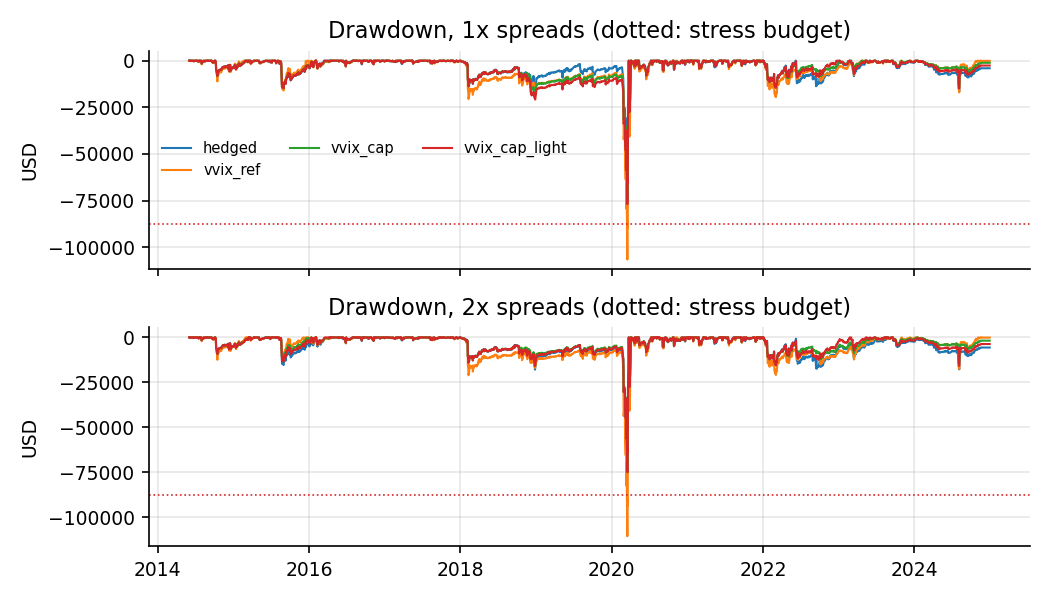
\includegraphics[width=0.92\linewidth]{figures/drawdown.png}\caption{Drawdown at 1x and 2x spreads}\end{figure}

Every book's worst drawdown runs from the same high (2 January 2018) to the same low (17 March 2020). The capped books start that fall from a lower high, because they made less in 2016-2017, and reach a lower low. The drawdown inside March 2020 itself is identical: \$67,552 at 1x and \$69,829 at 2x in all three books.

\begin{figure}[H]\centering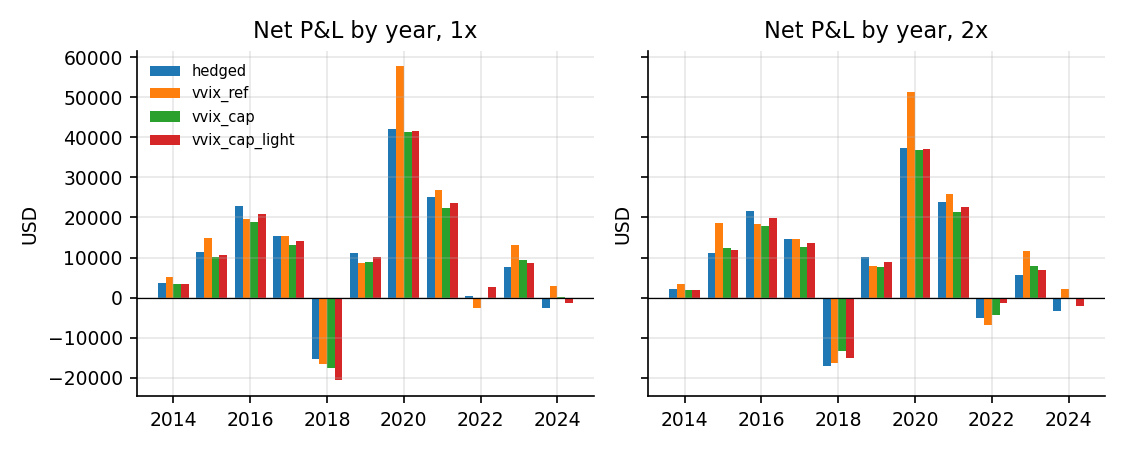
\includegraphics[width=0.92\linewidth]{figures/yearly.png}\caption{Net P\&L by year}\end{figure}

The cap costs a little in most years, about \$2-4k at 1x in 2016, 2017, 2018, 2019 and 2021. It gains in 2023 and 2024, when the fixed book lost money or made little. The 2018 difference changes sign between spreads: \ensuremath{-}\$2.4k at 1x and +\$3.8k at 2x.

\begin{figure}[H]\centering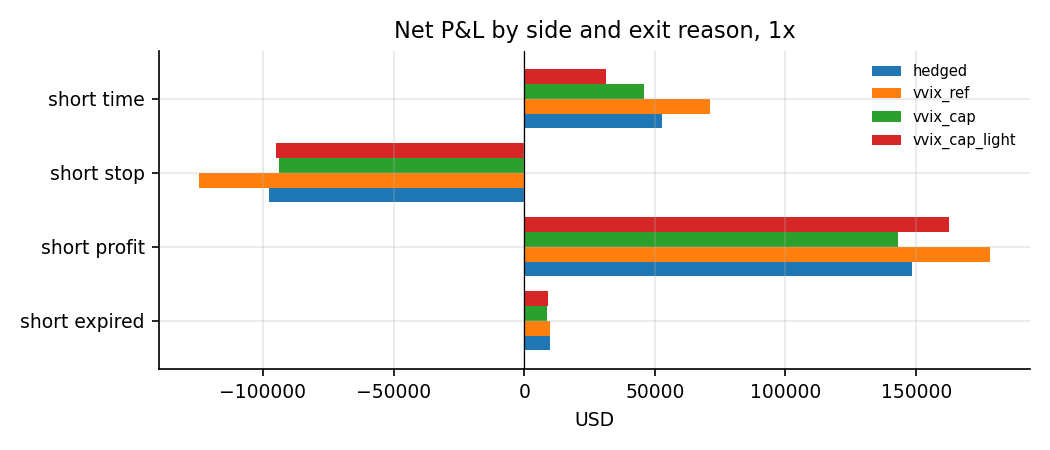
\includegraphics[width=0.92\linewidth]{figures/by_reason.png}\caption{Net P\&L by side and exit reason, 1x}\end{figure}

The cap makes every exit type smaller, profit-takes and stops alike. It barely changes which exits happen: one October 2018 trip moved from a time exit to a profit-take.

\begin{figure}[H]\centering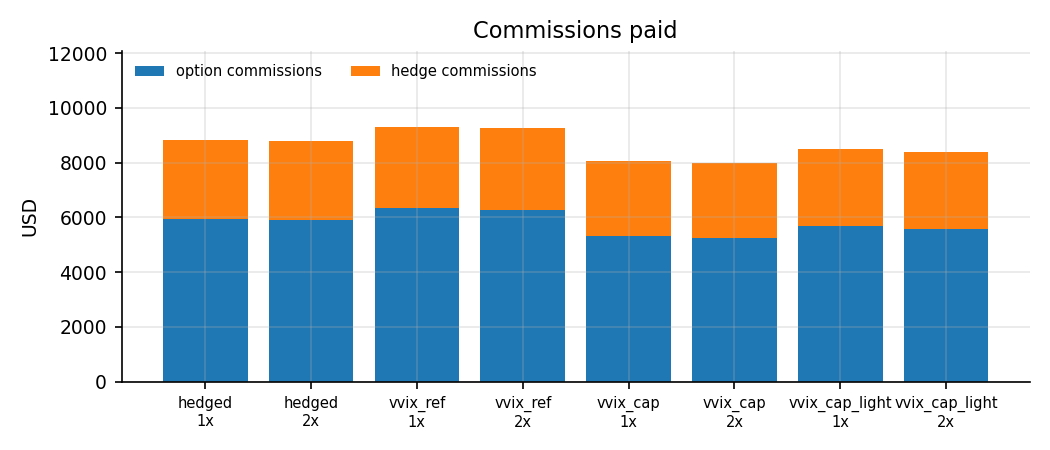
\includegraphics[width=0.92\linewidth]{figures/fees.png}\caption{Commissions paid}\end{figure}

Smaller entries cut option commissions by about \$600 at 1x. Hedge commissions barely change, because the daily hedge order count is about the same.

\begin{figure}[H]\centering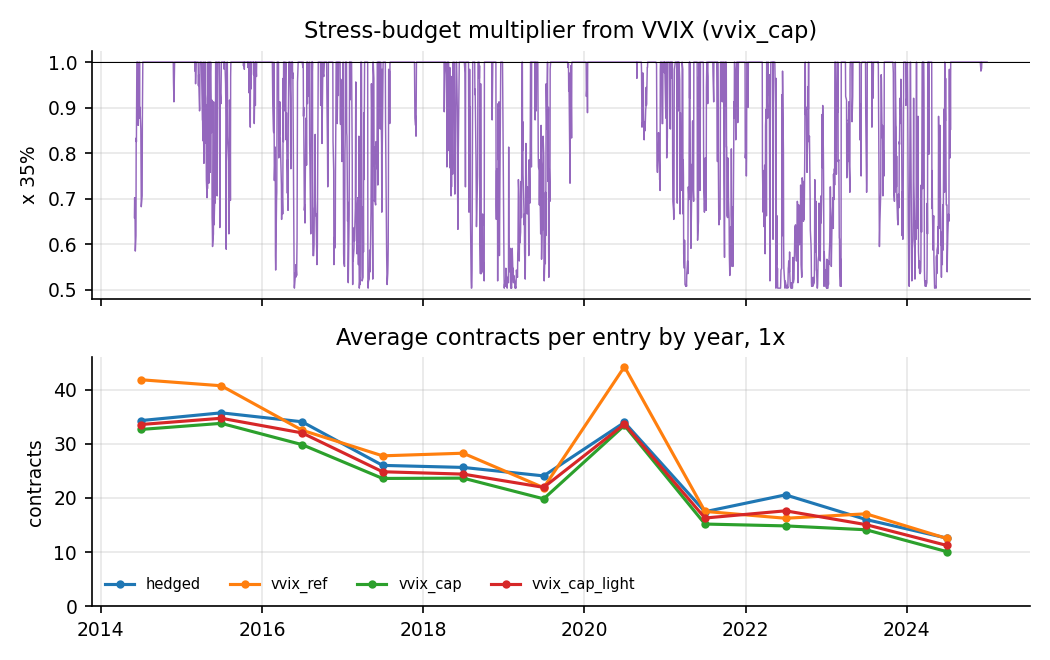
\includegraphics[width=0.92\linewidth]{figures/multiplier.png}\caption{Stress-budget multiplier from VVIX and contracts per entry}\end{figure}

The multiplier is below 1 on calm stretches, often reaching 0.5x in 2019, 2022 and 2024, and is 1 whenever VVIX is above its one-year median. Average contracts per entry are about 1.6-5.7 lower than the fixed budget's in every year except 2020 (0.6 lower).

\section{Analysis}

\textbf{The cap can't reach the crash.} Before the 2020 crash, VVIX was above its one-year median. So all six entries the capped book opened from February to April 2020 were sized at 1x, with the same contract counts as the fixed book (19, 27, 41, 100, 71 and 40). The March 2020 drawdown, which sets the book's maximum drawdown, is therefore unchanged. The rule can only cut size on calm days, and calm days are not where this book loses most. The 2020-2024 Sharpe check passes, but only just: the crash dominates that half, and the cap leaves it untouched.

\textbf{On calm days it cuts trades that were profitable.}

\begin{itemize}

\item 82 of the primary's 182 entries at 1x (45\%) were sized below 1x. The mean multiplier at entry was 0.88.

\item 171 of its round trips opened at the same time as one of the fixed book's.

\begin{itemize}

\item On the 73 matched trips that were cut, the fixed book made \$38.2k and the capped book \$32.8k. That \$5.4k drop is mechanical: same trades, fewer contracts.

\item The 98 matched trips that weren't cut differ by +\$3.4k. One October 2018 trip exited at a different time (+\$2.6k); hedge-share differences on the rest add \$0.8k.

\end{itemize}

\item The 11 round trips each book opened alone, from September 2018 to January 2019 and from June to October 2022, cost the capped book \$7.3k more (\ensuremath{-}\$11.7k against \ensuremath{-}\$4.5k). That is path dependence: a smaller position closed at a different time, and every later entry moved.

\item Cutting the low-VVIX trades lowered 2014-2019 P\&L from \$49.1k to \$36.7k at 1x without lowering the risk of that half much, so its Sharpe ratio fell from 0.84 to 0.66.

\item Per contract by VVIX tercile at entry, the fixed book made \$5.7 (low), \$25.7 (middle) and \ensuremath{-}\$0.1 (high), with the high tercile always at 1x. Low-VVIX entries were less profitable per contract than the middle tercile, but still positive (these are unweighted means; the high tercile made the most total net, \$55.8k). The cap took 7 contracts off them on average (22.2 to 15.0) and cut that tercile's net from \$20.4k to \$14.1k.

\end{itemize}

\textbf{Why the drawdown got deeper at 1x.} Both books' worst drawdown runs from 2 January 2018 to 17 March 2020. The capped book reached that high with \$45.5k instead of \$53.4k and ended at \ensuremath{-}\$29.5k instead of \ensuremath{-}\$17.0k. Over the drawdown it lost \$2.4k more in 2018, through the worse 1x path in Q4 2018, and made \$2.2k less in 2019, mostly in January as the Q4 2018 path unwound (entries in 2019 averaged 0.83x, but matched cut trips closing in 2019 differ by only \ensuremath{-}\$0.3k). So the drawdown measured from the 2018 high grew by \$4.6k.

\textbf{Why 2x passed and 1x did not.}

\begin{itemize}

\item At 2x the books diverged in different months. The 2x path through Q4 2018 matched the fixed book, and the unmatched trades fell in 2021-2022 instead.

\item At 2x the cut trades made about the same in both books (\$22.0k against \$21.9k). The 2x passes are by 0.01-0.03 of Sharpe and \$1.2k of drawdown.

\item This is the same kind of noise one changed exit creates. It is not evidence that the rule works at wider spreads.

\end{itemize}

\section{Verdict}

\textbf{Failed} on the pre-registered bar: three of the four checks fail at 1x.

Archive the capped VVIX tilt. Together with the uncapped card, the evidence is that VVIX does not rank this book's trades:

\begin{itemize}

\item sizing up on high VVIX was leverage on March 2020;

\item sizing down on low VVIX trims small but positive trades.

\end{itemize}

If the desk wants a smaller calm-period book, the 15\% and 25\% budgets in the crash-shock card are the direct test.

\section{Caveats}

\begin{itemize}

\item \textbf{In-sample:} the idea came from the 2026-11-02 VVIX sizing results on 2014-2024, including its per-contract P\&L by VVIX tercile, and the book was chosen after its 2014-2024 results.

\item \textbf{Path dependence:}

\begin{itemize}

\item About 6\% of round trips at 1x (11 of 182) differ between the books, and they move the 2014-2019 result by several thousand dollars.

\item The 1x and 2x results disagree on the drawdown, full-window Sharpe and 2014-2019 Sharpe checks for that reason.

\end{itemize}

\item \textbf{One crash:} the full-window drawdown of every book is set by March 2020, which the cap does not touch.

\item \textbf{VVIX and VIX move together}, so this test can't separate a VVIX effect from a vol-level effect.

\item \textbf{Spread model:} fitted on about two weeks of calm 2026 live quotes; the 2x run is the stress test. Fills of up to 100 contracts use the one-contract spread model.

\item \textbf{Margin} is not modelled.

\item \textbf{Data gaps:} about 3.3\% of scheduled times are skipped (no snapshot), plus 9 unfilled orders and 15 times without a delta per run.

\end{itemize}

\section{Trials}

4 trials for this experiment (2 variants \ensuremath{\times} 1x and 2x, one run of \texttt{experiment.\allowbreak{}py}), plus the baseline's 2.

\begin{itemize}

\item The reference \texttt{2026-\allowbreak{}10-\allowbreak{}22-\allowbreak{}stress-\allowbreak{}sized-\allowbreak{}puts/\allowbreak{}hedged} and the context \texttt{2026-\allowbreak{}11-\allowbreak{}02-\allowbreak{}vvix-\allowbreak{}sizing/\allowbreak{}vvix} runs were reused, not rerun.

\item The registry tags the runs \texttt{af47198-\allowbreak{}dirty} (\texttt{vvix\_\allowbreak{}cap}) and \texttt{3568520-\allowbreak{}dirty} (\texttt{vvix\_\allowbreak{}cap\_\allowbreak{}light}): pre-registration commits of parallel cards in the same batch, both made after this card's 6eae543. They are \texttt{-\allowbreak{}dirty} because the other cards' uncommitted files were in the shared working tree. This card's config, script, the engine and \texttt{backtest.\allowbreak{}toml} did not change between 6eae543 and those commits.

\item The pass bar was not changed.

\end{itemize}

\end{document}
